% !TEX root = thesis.tex

\chapter{Curriculum vitae}

\noindent
Gustavo Adolfo \href{http://ken.mx}{\textbf{Ken Arroyo Ohori}} was born on June 12, 1985 in Mexico City.
He graduated in 2003 from the Bicultural High School (`\emph{Preparatoria Bicultural}') programme and in 2007 from the BSc in Computer Science and Technology programme (`\emph{ITC01: Ingenier\'\i{}a en Tecnolog\'\i{}as Computacionales}') at the Mexico City campus of the Monterrey Institute of Technology and Higher Education (`\emph{Instituto Tecnol\'ogico y de Estudios Superiores de Monterrey}').

\marginpar{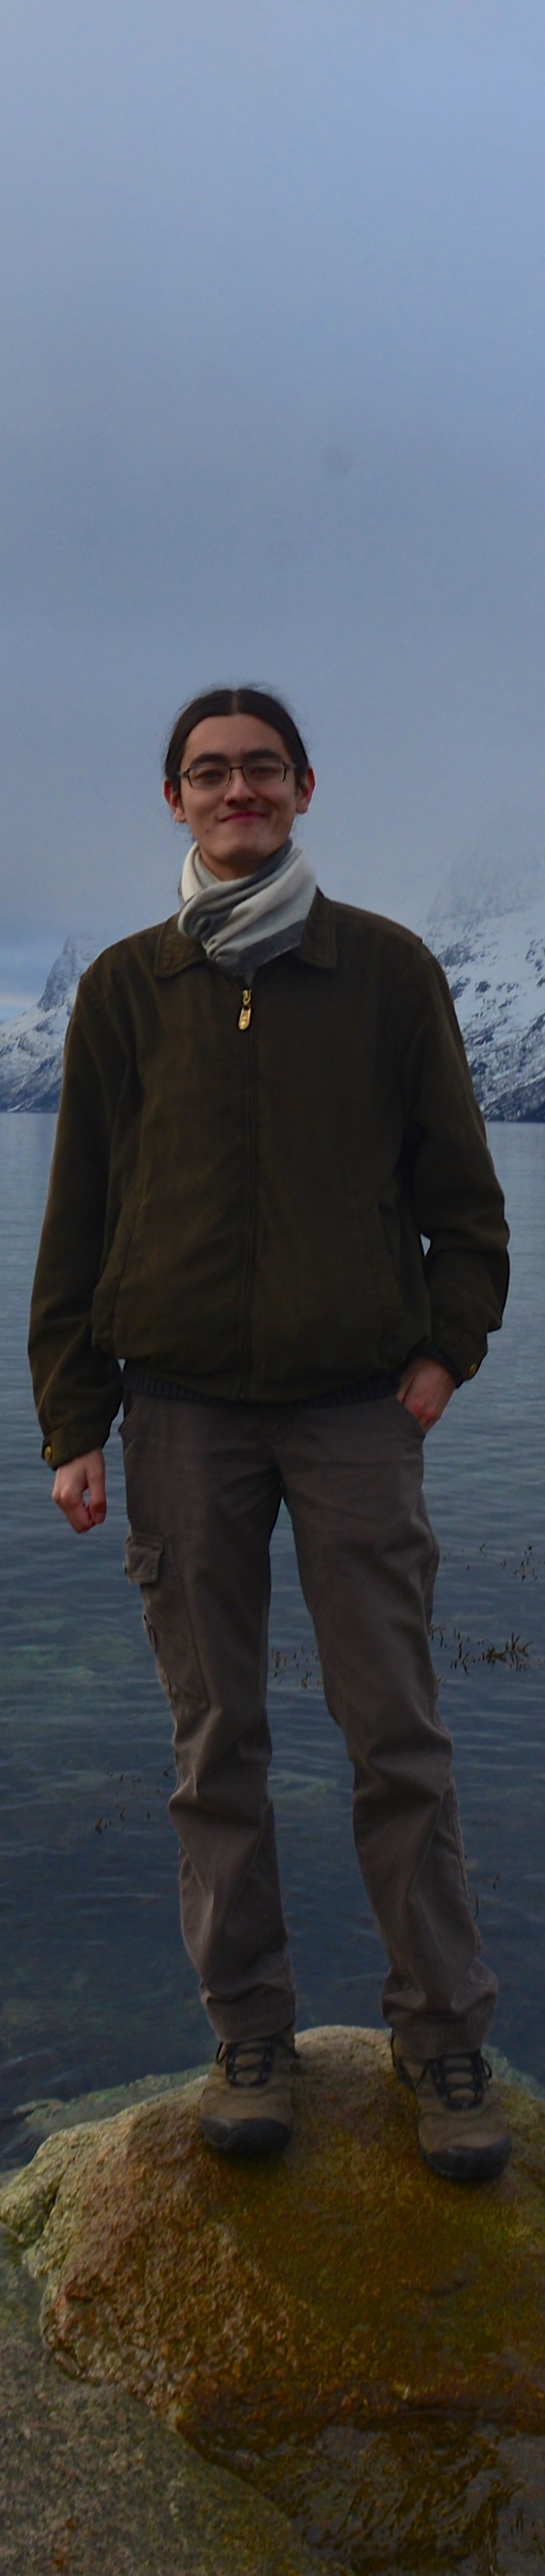
\includegraphics[width=\marginparwidth]{figs/me}}

Arriving to the Delft University of Technology in 2008, Ken graduated from the MSc in Geomatics programme in 2010 with his thesis on the \emph{Validation and automatic repair of planar partitions using a constrained triangulation}, which later evolved into some of the data repair ideas exposed in \refch{ch:cleaning} of this thesis.

In 2011, Ken started his PhD project on the \emph{Higher-dimensional modelling of geographic information}, supervised by \href{https://3d.bk.tudelft.nl/jstoter/}{Jantien Stoter} and \href{http://tudelft.nl/hledoux}{Hugo Ledoux}, working under the umbrella of the project \emph{5D Data Modelling: Full Integration of 2D/3D Space, Time and Scale Dimensions} of the Dutch Technology Foundation (\emph{STW}).
In October 2012, he visited \href{http://liris.cnrs.fr/guillaume.damiand/}{Guillaume Damiand}, collaborating on the incremental construction method that later became \refch{ch:incremental-construction} of this thesis.

In 2016, Ken started working as a postdoc in the same \emph{5D Data Modelling} project, focusing on 4D visualisation and in the integrated modelling of space and time.

\clearpage
\section*{Publications}

{\small
\begin{itemize}
\papermethodsxvoxelisation%
\paperijgisroeland%
\paperudmvobj%
\paperisprsnd%
\paperijgind\mparshift{-3.3\baselineskip}\marginpar{\raggedleft{}In \refch{ch:linking-lods}}%
\paperijgisextrusion\mparshift{-3.3\baselineskip}\marginpar{\raggedleft{}In \refch{ch:extrusion}}%
\paperijgisndstructures\mparshift{-3.3\baselineskip}\marginpar{\raggedleft{}In \refse{se:data-structures} \& \refse{se:nd-modelling-conclusions}}%
\papercgeoprepair\mparshift{-2.3\baselineskip}\marginpar{\raggedleft{}In \refse{se:pprepair}}%
\papericaaincrementalconstruction\mparshift{-6.3\baselineskip}\marginpar{\raggedleft{}In \refch{ch:incremental-construction}}%
\paperacmsigspatialextrusion%
\clearpage%
\papericcsand%
\papergeoadvancesnd\mparshift{-5.2\baselineskip}\marginpar{In \refse{se:duality}}%
\paperagileslicing%
\paperpfgpprepair\mparshift{-3.2\baselineskip}\marginpar{In \refse{se:pprepair}}%
\paperosgisrepair%
\papertdgeoinfond%
\paperagileprepair%
\paperostravaedgematching%
\end{itemize}
}

\clearpage
\null%
\marginpar{
\vspace*{13.5cm}

\includegraphics[width=\marginparwidth]{figs/3dgeoinfo}
}
